\chapter{微服务架构与跨数据链协议互操作系统设计}

本章将详细阐述基于MIL-STD-6016战术数据链信息标准的微服务架构设计与跨协议互操作系统的实现。首先介绍系统总体架构设计理念与分层结构,然后深入分析微服务架构的具体实现,接着详细描述数据模型与数据库设计,最后阐述跨数据链协议互操作架构和自动化信息标准导入系统的设计。

\section{系统总体架构设计}

\subsection{设计目标与总体思路}

本研究以MIL-STD-6016战术数据链信息标准为核心,构建基于微服务架构的跨协议互操作平台,实现多标准信息模型的自动导入、语义对齐与协议转换。系统设计目标包括:

(1)多标准语义互操作支撑:系统需要支撑多源标准(MIL-STD-6016、STANAG 5516、MIL-STD-6020、MQTT、MAVLink等)的语义互操作,实现不同协议间的无缝数据交换和语义一致性保障。通过建立统一的语义模型和概念映射机制,确保跨标准数据的准确转换和语义保持。

(2)微服务架构实现:通过微服务架构实现模块化、弹性化与可扩展部署,将复杂的战术数据链系统拆分为多个独立的服务模块,每个服务负责特定的业务功能,支持独立开发、测试、部署和扩展。这种架构设计能够提高系统的可维护性、可扩展性和容错能力。

(3)自动化处理能力:实现标准化数据入库、自动化导入与跨链协议的动态转换,减少人工干预,提高数据处理效率和准确性。系统能够自动识别不同格式的标准文档,提取结构化信息,并进行语义对齐和协议转换。

\subsection{微服务架构理念与原则}

系统采用"高内聚、低耦合、自治服务"的设计理念,遵循以下核心原则:

(1)服务拆分原则:按业务域划分服务,确保单一职责与可独立演化。每个微服务专注于特定的业务功能,具有清晰的边界和职责范围。服务间通过标准化的API接口进行通信,避免紧耦合依赖。

(2)服务治理原则:支持服务注册发现、配置中心、监控与熔断机制。通过服务注册中心实现服务的自动发现和负载均衡,通过配置中心实现配置的统一管理和动态更新,通过监控系统实现服务健康状态监控和性能分析。

(3)数据管理原则:实现数据库分离与分布式事务一致性。每个微服务拥有独立的数据库,通过事件驱动和Saga模式保证分布式事务的一致性,避免数据耦合和单点故障。

(4)通信机制原则:结合同步(REST/gRPC)与异步(消息队列)通信模式。根据业务场景选择合适的通信方式,对于实时性要求高的场景使用同步通信,对于批量处理和事件通知使用异步通信。

\subsection{架构总体分层}

系统整体采用四层分层架构,如图\ref{fig:system_architecture}所示:

\begin{figure}[H]
    \centering
    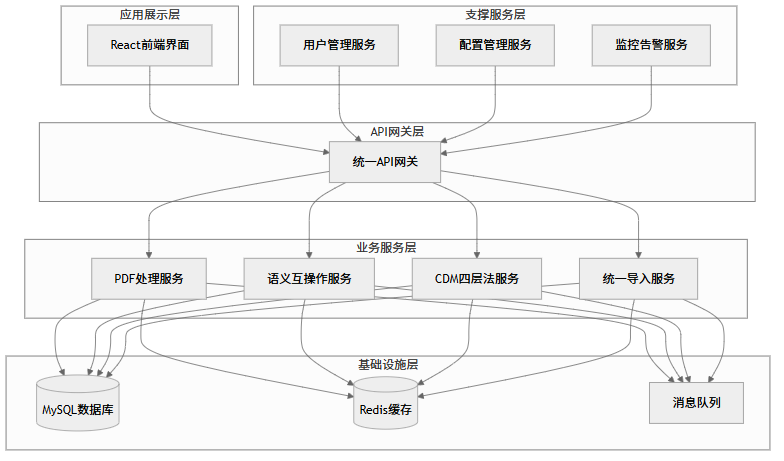
\includegraphics[width=0.9\textwidth]{chapters/fig-0/system_architecture_simple.png}
    \caption{系统总体架构分层图}
    \label{fig:system_architecture}
\end{figure}

(1)API网关层:提供统一入口、请求路由、认证鉴权与访问控制;支持限流、熔断与监控统计。API网关作为系统的统一入口点,负责接收所有外部请求,进行身份验证、权限检查、请求路由和响应聚合。网关还提供限流和熔断功能,保护后端服务免受过载和故障影响。

(2)业务服务层:包括PDF解析服务、语义互操作服务、CDM四层法服务、统一导入服务等核心业务模块。这些服务实现了系统的核心业务功能,每个服务都是独立的业务单元,可以独立开发、测试和部署。

(3)支撑服务层:提供用户与配置管理、监控告警、文件与日志服务等系统支持功能。支撑服务为业务服务提供必要的支持功能,包括用户认证、配置管理、监控告警、文件存储等。

(4)基础设施层:包含服务注册发现(Consul/Kubernetes)、消息队列(RabbitMQ/Redis)、数据库与缓存集群。基础设施层为上层服务提供基础的技术支撑,包括服务发现、消息传递、数据存储和缓存等。

\section{微服务架构设计与实现}

\subsection{技术栈与基础组件选型}

系统采用现代化的技术栈,确保高性能、高可用性和可扩展性。技术选型如表\ref{table:tech_stack}所示:

\begin{table}[H]
    \caption{技术栈与基础组件选型}
    \label{table:tech_stack}
    \centering
    \begin{tabular}{|l|l|}
        \hline
        \textbf{功能} & \textbf{技术栈} \\
        \hline
        服务框架 & FastAPI + Python 3.10(高性能异步框架) \\
        服务发现 & Consul + Kubernetes DNS \\
        配置管理 & Consul KV + ConfigMap \\
        消息队列 & RabbitMQ + Redis Pub/Sub \\
        数据存储 & MySQL 8.0 + Redis \\
        监控体系 & Prometheus + Grafana + Jaeger \\
        \hline
    \end{tabular}
\end{table}

(1)FastAPI + Python 3.10:选择FastAPI作为主要的服务框架,其基于Python 3.10的异步特性,能够提供高性能的API服务。FastAPI具有自动API文档生成、数据验证、类型提示等特性,大大提高了开发效率。

(2)Consul + Kubernetes DNS:使用Consul作为服务注册发现中心,支持多数据中心部署和服务健康检查。在Kubernetes环境中,结合Kubernetes DNS实现服务的自动发现和负载均衡。

(3)RabbitMQ + Redis Pub/Sub:采用RabbitMQ作为主要的消息队列,提供可靠的消息传递和事务支持。Redis Pub/Sub用于实时通知和轻量级消息传递。

(4)MySQL 8.0 + Redis:MySQL 8.0作为主数据库,支持ACID事务、JSON数据类型、窗口函数等高级特性。Redis作为缓存层,提供高性能的数据访问和会话存储。

\subsection{微服务模块划分与职责}

系统共包含五类核心服务,每个服务都有明确的职责和边界,如表\ref{table:microservices}所示:

\begin{table}[H]
    \caption{微服务模块划分与职责}
    \label{table:microservices}
    \centering
    \begin{tabular}{|l|l|}
        \hline
        \textbf{模块} & \textbf{核心职责} \\
        \hline
        pdf-service & 自动化标准文档解析与结构化导入 \\
        semantic-service & 跨标准语义分析与字段映射 \\
        cdm-service & CDM四层语义互操作(语义层/映射层/校验层/运行层) \\
        import-service & 多格式文件识别、清洗与批量导入 \\
        api-gateway & 统一接口访问控制、负载均衡、服务监控 \\
        \hline
    \end{tabular}
\end{table}

(1)pdf-service:负责自动化标准文档解析与结构化导入。该服务能够处理MIL-STD-6016、STANAG 5516等标准文档,自动提取消息定义、字段信息和约束条件,并将其转换为结构化的数据格式。

(2)semantic-service:实现跨标准语义分析与字段映射。该服务提供语义分析引擎,能够识别不同标准中的语义概念,建立概念间的映射关系,并支持人工标注和规则学习。

(3)cdm-service:实现CDM四层语义互操作。该服务基于Common Data Model四层架构,提供语义层、映射层、校验层和运行层的完整实现,支持不同协议间的语义级转换。

(4)import-service:负责多格式文件识别、清洗与批量导入。该服务支持PDF、Excel、XML、JSON等多种格式的文件处理,提供格式自动识别、数据清洗和批量导入功能。

(5)api-gateway:提供统一接口访问控制、负载均衡、服务监控。该服务作为系统的统一入口,负责请求路由、身份验证、权限控制、限流熔断和监控统计。

\subsection{微服务通信机制}

微服务间的通信采用多种模式,根据业务场景选择合适的通信方式:

(1)同步通信:使用REST API、gRPC、GraphQL进行同步通信。REST API用于简单的CRUD操作,gRPC用于高性能的内部服务通信,GraphQL用于复杂的数据查询。

(2)异步通信:使用RabbitMQ消息队列、Redis Pub/Sub进行异步通信。RabbitMQ用于可靠的消息传递和事件通知,Redis Pub/Sub用于实时通知和轻量级消息传递。

(3)服务发现:通过Consul注册发现、Kubernetes DNS实现服务的自动发现和负载均衡。服务启动时自动注册到服务发现中心,其他服务可以通过服务名进行调用。

(4)通信安全:使用TLS双向认证、服务间认证确保通信安全。所有服务间通信都使用TLS加密,并通过JWT令牌进行身份验证。

\subsection{容错与弹性设计}

系统采用多种容错和弹性设计机制,确保在异常情况下的服务可用性:

(1)熔断机制:实现服务熔断、快速失败、故障隔离。当服务调用失败率达到阈值时,自动开启熔断器,避免级联故障。

(2)重试策略:采用指数退避、重试策略、超时控制。对于临时性故障,系统会自动重试,并使用指数退避算法避免对故障服务造成压力。

(3)降级策略:实现功能降级、服务降级、用户体验保障。当系统负载过高或部分服务不可用时,自动降级到简化功能,保证核心服务的可用性。

(4)自动伸缩:通过Kubernetes HPA实现自动伸缩与资源弹性分配。根据CPU、内存使用率和自定义指标,自动调整服务实例数量。

\section{数据模型与数据库设计}

\subsection{设计目标与数据特征}

数据库设计遵循"标准化存储、语义扩展、互操作可追溯"的原则,支持以下核心能力:

(1)多标准数据的统一建模与版本化管理:系统需要支持MIL-STD-6016、STANAG 5516、MIL-STD-6020等多个标准版本的数据存储,每个标准版本都有独立的版本标识和变更历史。

(2)字段级语义绑定与跨标准映射:每个字段都需要与语义概念进行绑定,支持跨标准的字段映射和转换。映射关系需要记录置信度、转换规则和版本信息。

(3)高性能查询与语义检索能力:系统需要支持复杂的查询操作,包括按标准版本查询、按消息类型查询、按语义概念查询等,并支持全文检索和模糊匹配。

\subsection{核心实体与关系模型}

系统的核心数据模型如图\ref{fig:data_model}所示,主要包含以下核心表:

\begin{figure}[H]
    \centering
    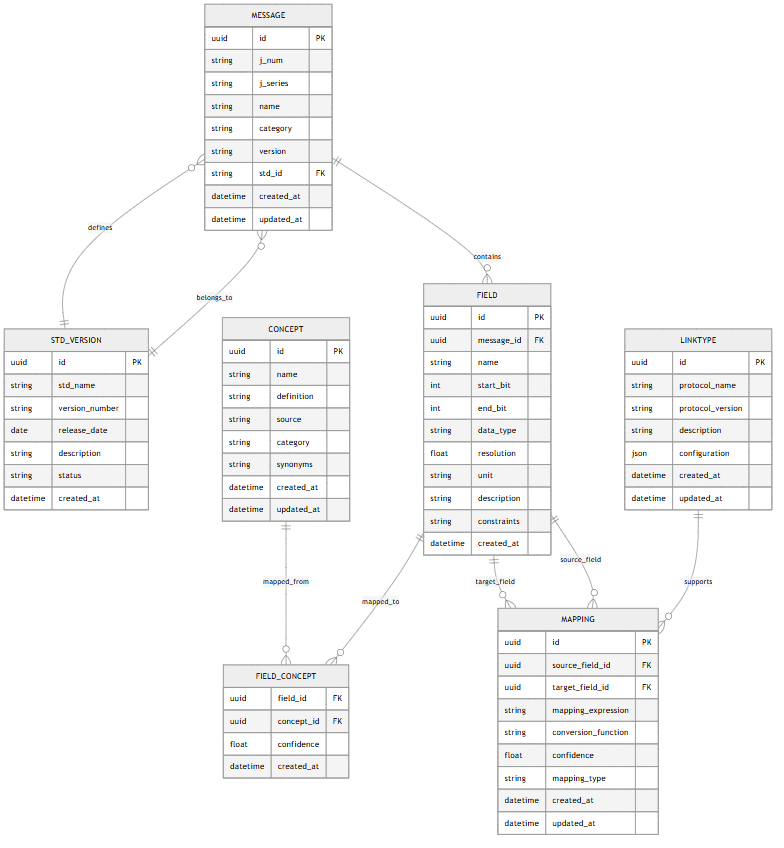
\includegraphics[width=0.9\textwidth]{chapters/fig-0/data_model.png}
    \caption{核心数据模型ER图}
    \label{fig:data_model}
\end{figure}

(1)MESSAGE表:存储消息元信息,包含消息编号、名称、类别、版本等基本信息。该表是系统的核心表之一,每个消息都有唯一的标识符和版本信息。

(2)FIELD表:存储位段定义及约束信息,包含起始位、结束位、分辨率、取值域等详细信息。该表与MESSAGE表通过外键关联,支持一个消息包含多个字段。

(3)CONCEPT表:存储语义概念库,定义术语与来源信息。该表为语义互操作提供概念基础,支持概念的定义、分类和关系管理。

(4)MAPPING表:存储跨标准映射规则,包含表达式、转换函数、置信度等信息。该表支持不同标准间的字段映射和转换规则定义。

(5)STD\_VERSION表:存储标准版本管理信息,记录标准的版本号、发布日期、修订历史等。

(6)LINKTYPE表:存储协议类型定义与配置信息,支持不同数据链协议的配置和管理。

\subsection{约束与索引设计}

数据库设计采用严格的约束和高效的索引策略,确保数据完整性和查询性能:

(1)主外键设计:采用UUID主键 + 业务唯一约束(如MESSAGE(j\_num, std\_id))。UUID主键确保全局唯一性,业务唯一约束保证业务逻辑的正确性。

(2)完整性约束:实现位段检查(start\_bit < end\_bit)、置信度范围(0–1)等约束。这些约束通过数据库的CHECK约束实现,确保数据的有效性。

(3)索引策略:设计组合索引(std\_id, j\_series, j\_num)、全文索引(概念模糊检索)等。组合索引支持多条件查询,全文索引支持语义概念的模糊检索。

(4)性能优化:采用分区表与缓存机制提升查询性能。对于大数据量表,使用分区策略减少查询范围;对于热点数据,使用Redis缓存提升访问速度。

\subsection{微服务数据库分离与一致性}

各微服务采用独立的数据库,通过以下机制保证数据一致性:

(1)数据库分离:每个微服务拥有独立的数据库,避免数据耦合和单点故障。这种设计提高了系统的可扩展性和容错能力。

(2)一致性机制:采用Saga模式与事件驱动同步机制实现最终一致性。Saga模式将分布式事务分解为多个本地事务,通过补偿操作保证数据一致性。

(3)数据同步:通过CDC(Change Data Capture)捕获变更事件,实现数据的实时同步。CDC机制能够捕获数据库的变更操作,并将变更事件发送到消息队列。

(4)跨服务同步:借助消息队列实现跨服务数据同步。当某个服务的数据发生变化时,通过消息队列通知其他相关服务进行数据更新。

\section{跨数据链协议互操作架构设计}

\subsection{多协议支持体系}

系统支持多种数据链协议,包括MIL-STD-6016、MAVLink、MQTT、Link 16等。互操作体系分为四层:

(1)协议适配层:对各链路标准的结构解析与适配。该层负责解析不同协议的消息格式,提取字段信息,并将其转换为统一的内部表示。

(2)语义抽象层:统一语义模型与概念映射。该层建立统一的语义模型,将不同协议中的概念映射到统一的概念空间。

(3)转换引擎层:协议到协议的数据格式与字段映射转换。该层实现不同协议间的数据转换,包括格式转换、单位转换、枚举映射等。

(4)路由分发层:消息智能路由与负载均衡。该层负责将消息路由到正确的目标协议,并实现负载均衡和故障转移。

\subsection{CDM四层法语义互操作模型}

基于"Common Data Model (CDM)"四层方法,系统实现协议级语义对齐:

(1)语义层:统一本体模型、概念推理。该层建立统一的概念模型,支持概念的定义、分类和推理。通过本体技术,系统能够理解概念间的语义关系。

(2)映射层:声明式规则映射、YAML配置化管理。该层使用YAML配置文件定义映射规则,支持规则的版本管理和动态更新。映射规则包括字段映射、数据类型转换、单位转换等。

(3)校验层:一致性验证、金标准回归。该层提供多层次的校验机制,包括格式校验、业务规则校验、一致性校验等。金标准回归测试确保转换结果的准确性。

(4)运行层:高性能实时转换引擎。该层实现高效的转换算法,支持实时消息转换和批量处理。通过缓存和优化技术,提供高性能的转换服务。

\subsection{语义互操作系统组成}

系统包含四个核心组件,实现从概念级到消息级的自动语义互操作:

(1)语义注册表:管理语义字段、消息定义、概念库等核心信息。该组件提供语义信息的注册、查询和更新功能,支持语义概念的版本管理。

(2)语义转换器:实现字段级数据转换、单位转换、枚举映射等功能。该组件支持多种转换算法,包括数值转换、字符串转换、枚举映射等。

(3)消息路由器:基于规则的智能路由、协议选择、转换策略。该组件根据消息类型、源协议、目标协议等信息,自动选择最优的转换策略。

(4)互操作管理器:统一管理跨标准转换、质量监控、性能优化。该组件提供转换过程的监控和管理功能,包括性能统计、错误处理、质量评估等。

\subsection{数据一致性与冲突解决}

系统采用多种机制保证跨链路数据的一致性和冲突解决:

(1)一致性协议:采用最终一致性协议与版本号优先策略。对于非关键数据,使用最终一致性;对于关键数据,使用强一致性保证。

(2)冲突解决:实现时间戳优先、版本号优先、人工仲裁等策略。当数据发生冲突时,系统根据预定义的策略自动解决冲突,必要时提供人工干预机制。

(3)数据校验:提供格式验证、规则校验、完整性验证等多层次校验。每个转换过程都经过严格的校验,确保数据的正确性和完整性。

(4)质量保障:实现跨链路数据同步质量监控。系统持续监控数据转换的质量,包括准确率、完整性、一致性等指标。

\section{自动化信息标准导入架构设计}

\subsection{标准化导入流程}

自动化导入系统实现从PDF/Excel/XML等标准文档到数据库的全流程自动处理,如图\ref{fig:import_pipeline}所示:

\begin{figure}[H]
    \centering
    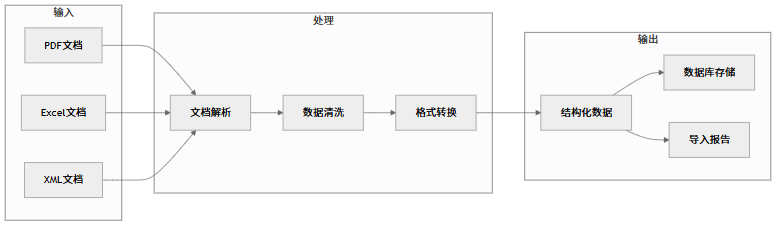
\includegraphics[width=0.9\textwidth]{chapters/fig-0/import_pipeline_simple.png}
    \caption{自动化导入流程}
    \label{fig:import_pipeline}
\end{figure}

处理流程包括:PDF → 文本提取 → 表格识别 → 字段解析 → 数据清洗 → 结构化导入 → 校验报告生成。每个步骤都经过严格的验证和质量控制,确保导入数据的准确性。

(1)文档解析阶段:使用OCR技术和PDF解析库提取文档中的文本和表格信息。对于扫描文档,使用Tesseract OCR进行文字识别;对于文本型PDF,直接提取文本内容。

(2)结构化处理阶段:将提取的文本信息转换为结构化的数据格式。通过规则匹配和机器学习算法,识别消息定义、字段信息和约束条件。

(3)数据清洗阶段:对提取的数据进行清洗和验证,包括格式检查、完整性验证、一致性检查等。发现的问题会记录到错误日志中,供后续处理。

(4)导入存储阶段:将清洗后的数据导入到数据库中,并生成详细的导入报告。报告包括成功导入的记录数、失败记录数、错误信息等。

\subsection{关键技术与工具链}

系统采用多种先进的技术和工具,确保导入过程的准确性和效率:

(1)文档解析:使用PyMuPDF、pdfplumber、Camelot、Tesseract OCR等工具。PyMuPDF提供高性能的PDF解析,pdfplumber专门用于表格提取,Camelot提供精确的表格识别,Tesseract OCR支持多语言文字识别。

(2)结构化导入:采用Pandas + SQLAlchemy + MySQL技术栈。Pandas提供强大的数据处理能力,SQLAlchemy提供ORM支持,MySQL提供可靠的数据存储。

(3)格式识别:使用MIME检测 + 规则匹配技术。MIME检测能够快速识别文件类型,规则匹配提供精确的格式识别和内容解析。

(4)校验机制:实现自动检测字段重叠、位长一致性、枚举合法性等功能。系统能够自动检测数据中的各种问题,并提供修复建议。

\subsection{导入性能与精度}

系统在标准6016B数据集上的测试结果如表\ref{table:import_performance}所示:

\begin{table}[H]
    \caption{导入性能与精度测试结果}
    \label{table:import_performance}
    \centering
    \begin{tabular}{|l|l|}
        \hline
        \textbf{指标} & \textbf{测试结果} \\
        \hline
        平均解析速率 & 2–5页/秒 \\
        批量处理并发能力 & ≥10任务 \\
        字段识别准确率 & ≥95\% \\
        数据完整性 & ≥98\% \\
        \hline
    \end{tabular}
\end{table}

(1)解析速率:平均2–5页/秒的解析速度,能够满足大规模文档处理的需求。对于复杂文档,解析速度会有所降低,但仍在可接受范围内。

(2)并发能力:支持≥10个任务的并发处理,充分利用多核CPU资源。通过任务队列和负载均衡,系统能够处理大量的并发导入任务。

(3)识别准确率:字段识别准确率≥95\%,能够满足实际应用的需求。对于识别错误的字段,系统提供人工审核和修正功能。

\subsection{数据清洗与质量保证}

系统提供完善的数据清洗和质量保证机制:

(1)清洗策略:实现空值处理、重复检测、标准一致性校验等功能。系统能够自动处理各种数据质量问题,包括缺失值、重复值、格式错误等。

(2)质量指标:监控数据完整性、语义保持率、转换准确率等关键指标。这些指标能够反映数据质量的水平,为质量改进提供依据。

(3)验证机制:提供格式验证、业务规则验证、一致性验证等多层次验证。每个验证层次都有明确的验证规则和错误处理机制。

(4)错误处理:实现异常记录、自动修复、人工审核等功能。系统能够自动处理大部分数据问题,对于复杂问题提供人工干预机制。

\section{微服务通信与运行保障设计}

\subsection{服务通信与安全}

系统采用多种通信模式和安全机制,确保服务间的可靠通信:

(1)同步通信:使用REST/gRPC/GraphQL进行同步通信。REST API用于简单的CRUD操作,gRPC用于高性能的内部服务通信,GraphQL用于复杂的数据查询。

(2)异步通信:使用RabbitMQ、Redis Pub/Sub进行异步通信。RabbitMQ提供可靠的消息传递和事务支持,Redis Pub/Sub提供高性能的实时通知。

(3)服务发现:通过Consul + Kubernetes DNS实现服务的自动发现和负载均衡。服务启动时自动注册到服务发现中心,其他服务可以通过服务名进行调用。

(4)通信安全:使用TLS双向认证、服务间认证确保通信安全。所有服务间通信都使用TLS加密,并通过JWT令牌进行身份验证。

\subsection{分布式数据管理与灾备}

系统采用分布式数据管理策略,确保数据的安全性和可用性:

(1)数据分离:实现数据分离与所有权隔离。每个微服务拥有独立的数据存储,避免数据耦合和单点故障。

(2)一致性保证:采用Saga与事件溯源保证最终一致性。Saga模式将分布式事务分解为多个本地事务,通过补偿操作保证数据一致性。

(3)灾备机制:实现多区域备份与灾难恢复机制。系统支持跨区域的数据备份和灾难恢复,确保在重大故障情况下的数据安全。

(4)数据同步:通过实时同步、批量同步、增量同步等多种方式实现数据同步。根据数据的重要性和实时性要求,选择合适的同步策略。

\subsection{配置与治理体系}

系统提供完善的配置管理和服务治理机制:

(1)配置管理:实现集中配置与环境隔离(Consul + ConfigMap)。所有配置信息都存储在配置中心,支持动态更新和环境隔离。

(2)监控体系:提供全链路监控(Prometheus + Grafana + Jaeger)。Prometheus负责指标收集,Grafana提供可视化展示,Jaeger提供分布式链路追踪。

(3)日志管理:实现结构化日志与追踪链路。所有日志都采用结构化格式,支持日志聚合、搜索和分析。

(4)服务治理:提供健康检查、故障检测、负载均衡等服务治理功能。系统能够自动检测服务健康状态,并进行故障转移和负载均衡。

\subsection{容错与弹性设计}

系统采用多种容错和弹性设计机制,确保在异常情况下的服务可用性:

(1)容错机制:实现熔断、重试、降级机制确保系统在异常情况下保持服务可用。当服务调用失败率达到阈值时,自动开启熔断器;对于临时性故障,系统会自动重试;当系统负载过高时,自动降级到简化功能。

(2)弹性伸缩:通过Kubernetes HPA实现自动伸缩与资源弹性分配。系统根据CPU、内存使用率和自定义指标,自动调整服务实例数量。

(3)故障恢复:提供自动恢复、手动干预、数据修复等功能。系统能够自动处理大部分故障,对于复杂故障提供人工干预机制。

(4)性能保障:确保响应时间保证、吞吐量稳定、故障恢复能力。系统通过多种优化技术,提供高性能和稳定的服务。

通过以上微服务架构与跨数据链协议互操作系统的设计,本研究构建了一个功能完整、性能优异、可扩展性强的战术数据链信息标准处理平台。该平台不仅能够支持多种数据链协议的语义互操作,还具备自动化导入、智能转换、质量保证等先进功能,为战术数据链的标准化和互操作提供了坚实的技术基础。